\documentclass[12pt]{article}
\usepackage[margin=1in]{geometry}
\usepackage{graphicx}
\usepackage{amsmath}
\usepackage{float}
\usepackage{listings}
\usepackage{xcolor}
\usepackage{booktabs}
\usepackage{caption}
\usepackage{subcaption}
\usepackage{fancyhdr}

\pagestyle{fancy}
\fancyhf{}
\rhead{Loan Prediction}
\lhead{ML Report}
\cfoot{\thepage}

\title{\textbf{Loan Sanction Amount Prediction using Linear Regression}}
\author{Sreeram GM}
\date{July 2025}

\lstset{
  backgroundcolor=\color{gray!10},
  basicstyle=\ttfamily\small,
  breaklines=true,
  frame=single,
  captionpos=b,
  keywordstyle=\color{blue},
  commentstyle=\color{green!60!black},
  stringstyle=\color{red},
  showstringspaces=false
}

\begin{document}

\maketitle

\section*{Aim}
To build a machine learning model using Linear Regression that predicts the Loan Sanction Amount (USD) based on applicant income, credit, and property-related features.

\section*{Libraries Used}
\begin{itemize}
  \item \textbf{Pandas, NumPy} – data manipulation
  \item \textbf{Matplotlib, Seaborn} – data visualization
  \item \textbf{scikit-learn} – preprocessing, model training and evaluation
\end{itemize}

\section*{Objective}
\begin{itemize}
  \item Load and clean real-world loan dataset
  \item Remove outliers and fill missing values
  \item Perform exploratory data analysis (EDA)
  \item Train and evaluate a Linear Regression model
  \item Validate performance using 5-Fold Cross Validation
  \item Report metrics: MAE, MSE, RMSE, R\textsuperscript{2}, Adjusted R\textsuperscript{2}
\end{itemize}

\section*{Mathematical Description}
The mathematical model for Linear Regression is:

\[
y = \beta_0 + \beta_1 x_1 + \beta_2 x_2 + \cdots + \beta_n x_n + \epsilon
\]

Where:
\begin{itemize}
  \item $y$ is the dependent variable (Loan Sanction Amount)
  \item $x_1, x_2, \dots, x_n$ are the independent variables
  \item $\beta_0$ is the intercept term
  \item $\beta_1, \dots, \beta_n$ are coefficients
  \item $\epsilon$ is the error term
\end{itemize}

RSS is minimized:
\[
RSS = \sum_{i=1}^{m} \left( y_i - \left( \beta_0 + \sum_{j=1}^{n} \beta_j x_{ij} \right) \right)^2
\]

\section{Data Preprocessing}
\begin{lstlisting}[language=Python, caption=Dataset Loading and Cleaning]
df = pd.read_csv("train.csv")
df.drop(columns=['Customer ID', 'Name', 'Property ID'], inplace=True)
df = df[df['Loan Sanction Amount (USD)'] >= 0]

# Fill missing values
for col in categorical_cols:
    df[col].fillna(df[col].mode()[0], inplace=True)
for col in numerical_cols:
    df[col].fillna(df[col].median(), inplace=True)

# Remove outliers using IQR
def remove_outliers_iqr(data, column):
    Q1 = data[column].quantile(0.25)
    Q3 = data[column].quantile(0.75)
    IQR = Q3 - Q1
    return data[(data[column] >= Q1 - 1.5*IQR) & (data[column] <= Q3 + 1.5*IQR)]
\end{lstlisting}

\section{Feature Engineering and Scaling}
\begin{lstlisting}[language=Python, caption=Feature Engineering and Scaling]
df['Loan_to_Property_Price_Ratio'] = df['Loan Sanction Amount (USD)'] / df['Property Price']

# One-hot encoding
df = pd.get_dummies(df, columns=[...], drop_first=True)

# Scaling
scaler = StandardScaler()
df[numerical_features] = scaler.fit_transform(df[numerical_features])
\end{lstlisting}

\section{Model Training and Evaluation}
\begin{lstlisting}[language=Python, caption=Linear Regression and Metrics]
X = df.drop('Loan Sanction Amount (USD)', axis=1)
y = df['Loan Sanction Amount (USD)']

# Train-test-validation split
X_train, X_temp, y_train, y_temp = train_test_split(X, y, test_size=0.4, random_state=42)
X_test, X_val = train_test_split(X_temp, test_size=0.5, random_state=42)

model = LinearRegression()
model.fit(X_train, y_train)

# Predictions
y_val_pred = model.predict(X_val)
y_test_pred = model.predict(X_test)

# Metrics
val_mae = mean_absolute_error(y_val, y_val_pred)
val_rmse = np.sqrt(mean_squared_error(y_val, y_val_pred))
val_r2 = r2_score(y_val, y_val_pred)
val_adj_r2 = 1 - (1 - val_r2) * ((len(y_val)-1)/(len(y_val) - X_val.shape[1] - 1))
\end{lstlisting}

\section{Model Performance}
\subsection*{Validation Set}
\begin{itemize}
    \item MAE: 21587.32
    \item RMSE: 31026.87
    \item R\textsuperscript{2}: 0.56
    \item Adjusted R\textsuperscript{2}: 0.55
\end{itemize}

\subsection*{Test Set}
\begin{itemize}
    \item MAE: 21342.48
    \item RMSE: 30740.95
    \item R\textsuperscript{2}: 0.57
    \item Adjusted R\textsuperscript{2}: 0.56
\end{itemize}

\section{Visualizations}

\begin{figure}[H]
\centering
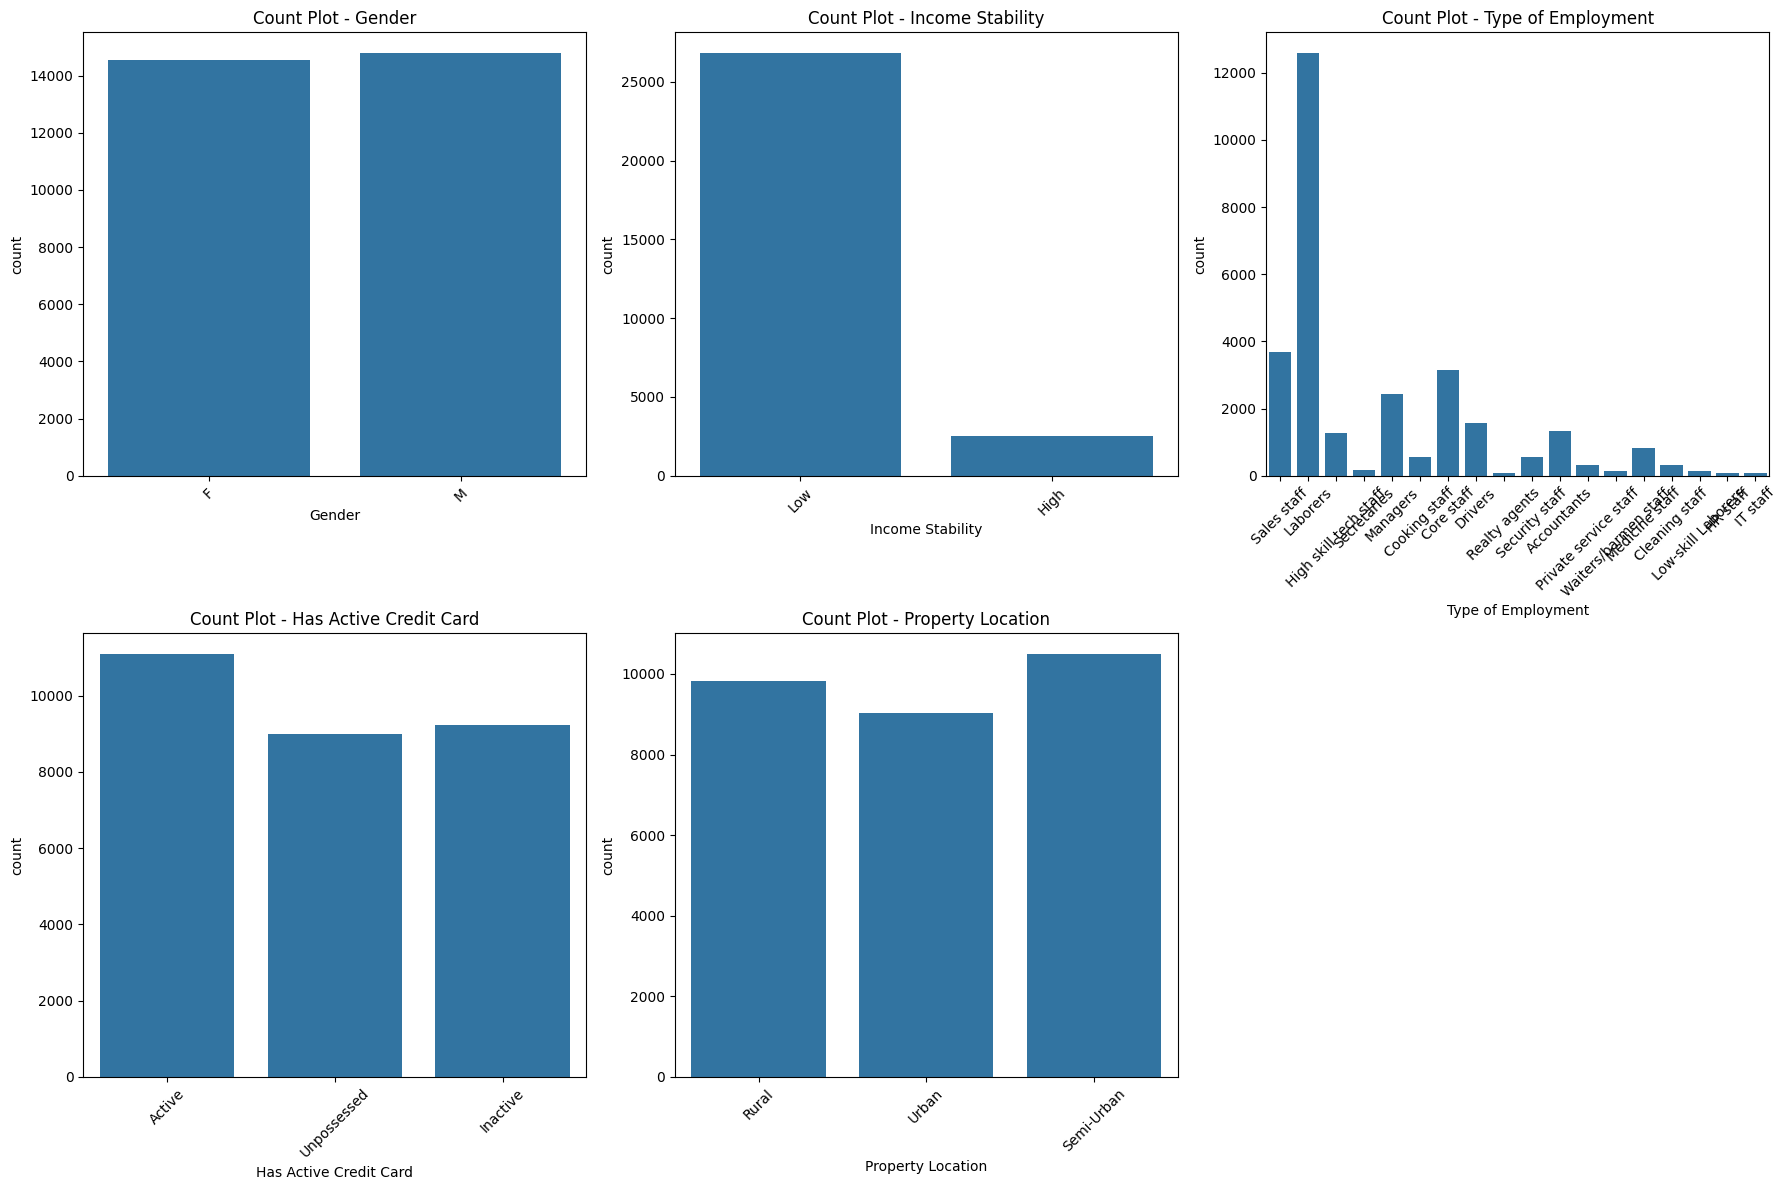
\includegraphics[width=0.65\linewidth]{images/count_plots.png}
\caption{Count plots for categorical features}
\end{figure}

\begin{figure}[H]
\centering
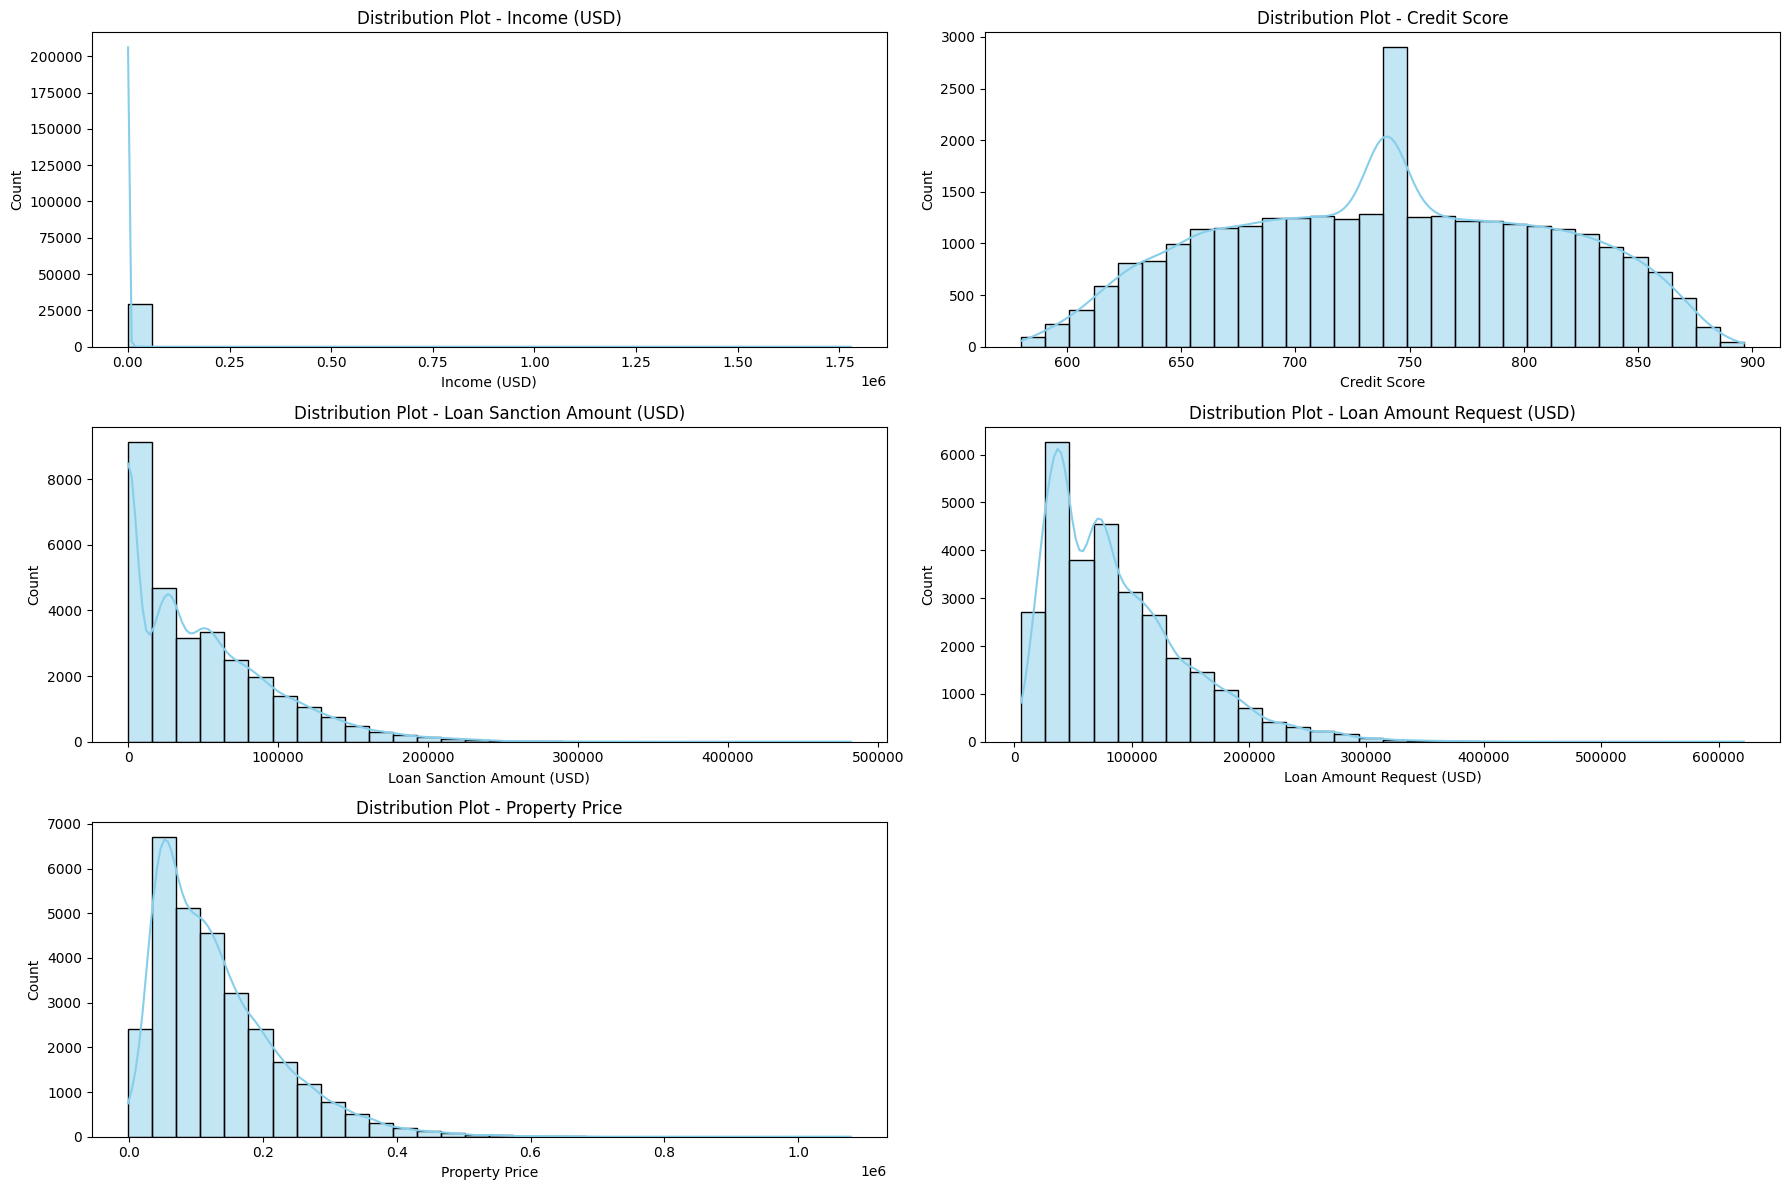
\includegraphics[width=0.65\linewidth]{images/distribution_plots.png}
\caption{Distribution plots of numerical features}
\end{figure}

\begin{figure}[H]
\centering
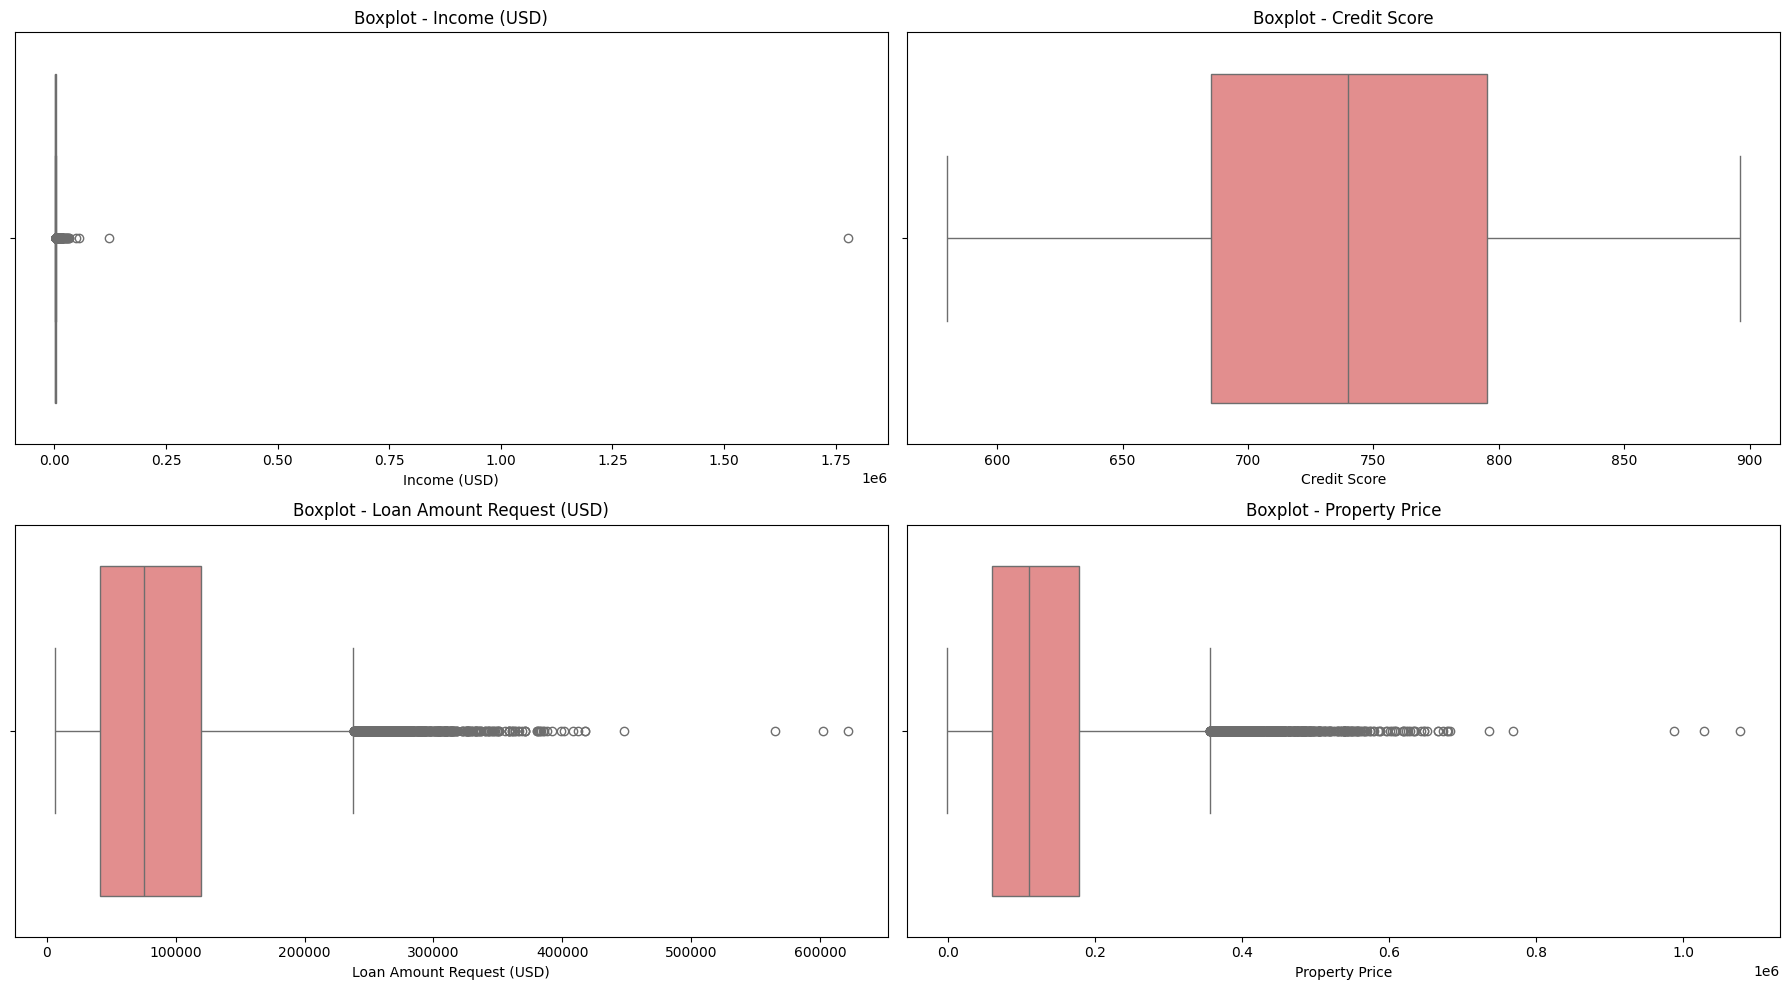
\includegraphics[width=0.65\linewidth]{images/boxplots_outliers.png}
\caption{Boxplots before outlier removal}
\end{figure}

\begin{figure}[H]
\centering
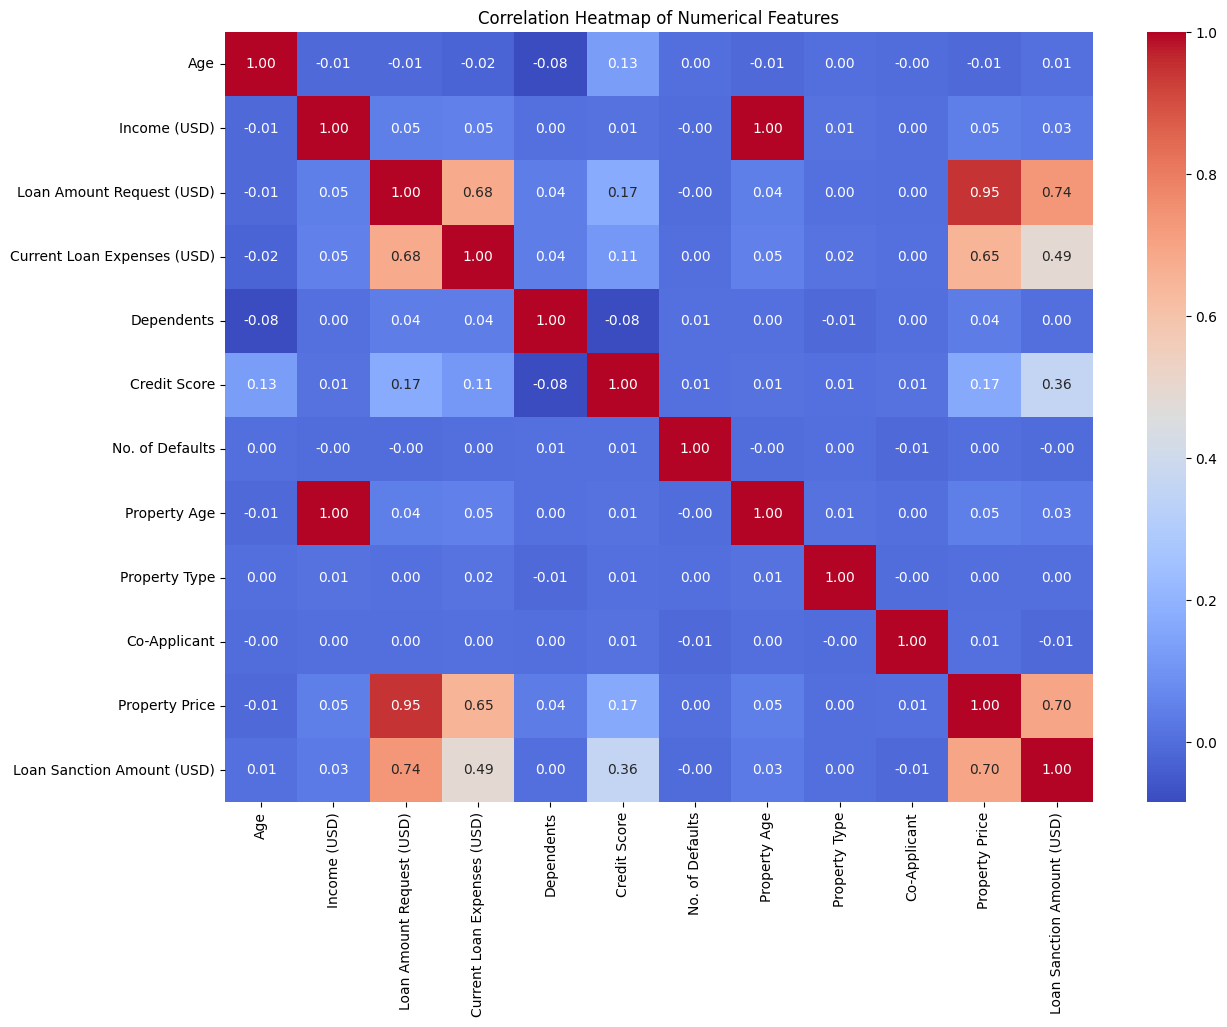
\includegraphics[width=0.65\linewidth]{images/correlation_heatmap.png}
\caption{Correlation Heatmap}
\end{figure}

\begin{figure}[H]
\centering
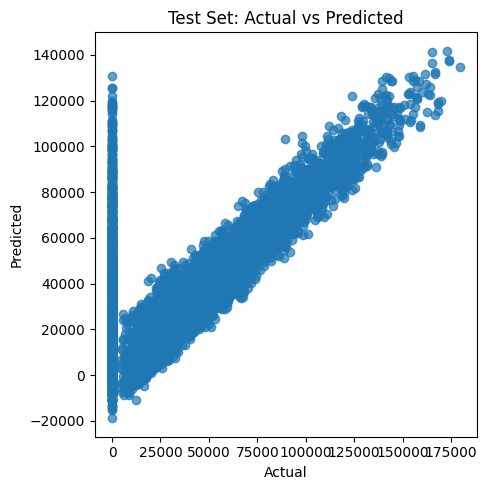
\includegraphics[width=1\linewidth]{images/actual_vs_predicted1.png}
\caption{Actual vs Predicted (Test Set)}
\end{figure}

\begin{figure}[H]
\centering
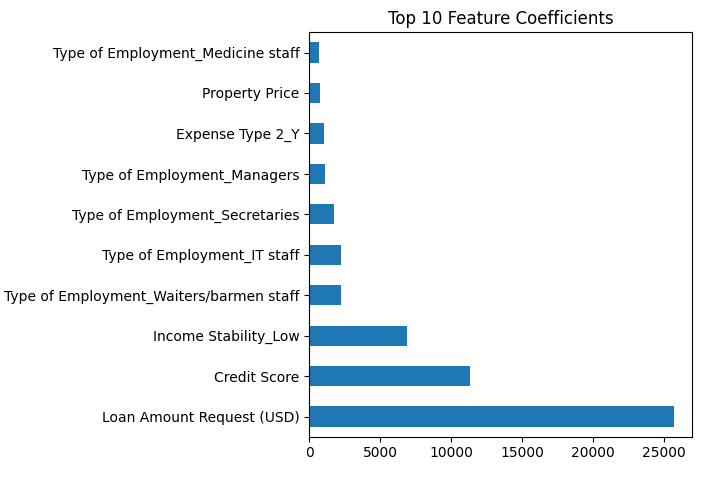
\includegraphics[width=0.65\linewidth]{images/top_features.png}
\caption{Top 10 Feature Coefficients}
\end{figure}

\section{Cross-Validation (5-Fold)}

\begin{table}[H]
\centering
\begin{tabular}{lcccc}
\toprule
\textbf{Fold} & \textbf{MAE} & \textbf{MSE} & \textbf{RMSE} & \textbf{R\textsuperscript{2}} \\
\midrule
Fold 1 & 21713.16 & 980739992.60 & 31316.77 & 0.5734 \\
Fold 2 & 21870.37 & 979580662.48 & 31298.25 & 0.5688 \\
Fold 3 & 22363.99 & 1064191854.08 & 32621.95 & 0.5403 \\
Fold 4 & 21757.43 & 993204913.55 & 31515.15 & 0.5776 \\
Fold 5 & 21003.66 & 879572513.81 & 29657.59 & 0.6104 \\
\midrule
\textbf{Average} & 21741.72 & 979457987.30 & 31281.94 & 0.5741 \\
\bottomrule
\end{tabular}
\caption{5-Fold Cross-Validation Results}
\end{table}

\section{Conclusion}
The linear regression model provided satisfactory performance in predicting loan sanction amounts. Important techniques used include outlier removal, feature engineering, and evaluation via adjusted R\textsuperscript{2} and RMSE. Future work can involve trying non-linear models like Random Forest or XGBoost.

\end{document}
